%Chapter 4

\chapter{Application} % Main chapter title

\section{Introduction}
Nous allons commencer par aborder, dans ce chapitre, quelques détails techniques concernant notre implémentation. Ensuite, nous présenterons l'interface que nous avons conçu pour l'application de notre approche. Enfin, nous examinerons plus en détails certains exemples de résultats de recherches pour des images précises.

\section{Technologie utilise}

Nous avons implémenté nos approches en langage Python (3.0) a l'aide de diffèrent Framework et bibliothèques.

\subsection{Pourquoi python?}
Nous avons choisi le langage pour différentes raisons dont:

\begin{itemize}
\item Le fait qu'il soit très simple et son niveau d'abstraction nous permet de mettre en place des prototype et de les tester rapidement.

\item Sa syntaxe (indentation obligatoire, entre autre) rend le code trivialement lisible.

\item L'existance de beacoup de librairie puissantes.

\item Ainsi qu'une communauté immense, une documentation tes importante une obtention d'aide très facile.
\end{itemize}


\subsection{Theano:}
Theano est le framework le plus utilisé, il est un des plus ancien et du coup, beaucoup de recherches se sont déjà basées dessus. 

Il a été conçu par le laboratoire MILA (Montreal Institute for Learning Algorithms) de l’Université de Montreal. C'est un projet Open Source que de nombreuse autre chercheurs de diffèrent laboratoires et institutions ont fini par rejoindre (Google Deepmind, New  York  University, NVIDIA Corporate, Meiji  University Tokyo ..etc ) [Theano 16].

Ce framework permet de définir des expressions mathématiques symboliques en les représentant par des graphes orientés acycliques. Ses derniers sont constitués de deux types de nœuds: \textbf{Variable} qui représentes les données et \textbf{Appliquer} qui représentes les opérations mathématiques. Cette représentation permet une manipulation simple des expressions dont, entre autre, la génération automatique de leurs dérivés.\\

Par exemple, si on défini un "scalar" x: \\

>> x = theano.dscalar('x')\\

ensuite une expression: \\

>> y = x ** 2\\

Si on se décide de visualiser le graph généré pour y :\\

>> theano.printing.pydotprint(y, outfile="yGraph.png", var\_with\_name\_simple=True)\\

\begin{figure}[H]
	\centering
		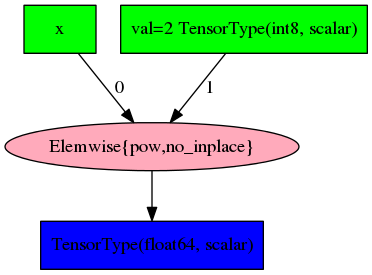
\includegraphics[width=3in]{Figures/yGraph.png}
	\caption[TheanoGraph]{Visualisation du graph d'une fonction}
	\label{fig:Electron}
\end{figure}

La dérivations automatiques s'effectue simplement en appliquant une fonction (grad). 
Donc, la dérivée de \textbf{y}, défini ci-dessus, par rapport a \textbf{x} peut être calcule avec: \\

>> gy = T.grad(y, x)\\

\textbf{gy} contient dorénavant la dérivée de \textbf{y} qui n'est rien d'autre que \textbf{2x} .\\

>> theano.pp(gy)\\
 '((fill((x ** TensorConstant{2}), TensorConstant{1.0}) * TensorConstant{2}) * (x ** (TensorConstant{2} - TensorConstant{1})))'\\
 

Une notion importante est celle de \textit{variables symboliques} qui représente des variables symboliques. Elle peuvent être considéré comme des buffers qui contient des valeurs qui peuvent être partagée entre plusieurs fonctions de Theano.\\

Un autre point fort est l'optimisation pour l'utilisation de matrice multi-dimensionnel, mais aussi la facilite de compiler les opérations sur des GPU.\\

Theano fut suivit d'autre framework qui ont repris les mêmes principes, l'un des plus connues étant Tensorflow de Google.

\subsection{Autre}
D'autre outils ajoutent des couches d'abstraction a Theano pour faciliter son utilisation (ex: Blocks, Lasagne, Keras) .
Le modèle (VGG CNN S) que nous avons utilisé est implémenté en Lasagne après avoir été convertie de Caffe (Caffe étant un autre Framework en C++ developpé par le laboratoire Berkeley Vision and Learning Center).\\

Pour les autoencoders, nous avons utilisé Blocks [Bart et al. 15], un autre framework theano qui facilite la définition de modèles et leur modification. Il introduit des outils pour l'apprentissage, visualisations et sérialisation. Enfin, Fuel permet formater les données d'apprentissage d'une façon a faciliter leur manipulation, surtout quand les tailles de ses dernières deviennent importantes.
Développés aussi par le laboratoire MILA, ces deux outils forment une base solide pour le développement de d’approche basé sur l'apprentissage profond.

\section{Interface}

Pour développer l'interface graphique nous avons utilise PyQt4, un module pour python qui permet de le lier avec Qt, un framework pour le développement d'application multi-plates-formes.\\

Nous allons montrer l'interface que nous avons développer pour l'application de notre approche.


\section{Tests}

Nous avons pris quelques images pour effectuer des testes sur les bases de donne WONG et AUTRE.

\section{Conclusion}

Nous concluons ce chapitre.
